\documentclass[tikz]{standalone}

\usepackage{tikz}

\begin{document}
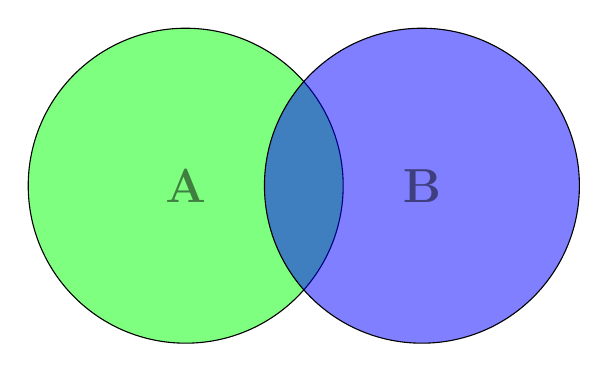
\begin{tikzpicture}
    %% You can adjust the opacity here. For venn diagrams it is convenient to have a low opacity so that you can see intersections
        \begin{scope} [fill opacity = 0.5]
    %% The draw command knows a lot of shapes. To make a rectangle you just need to specify two diagonal corners. Make sure you always have a semicolon at the end of your draw commands, otherwise latex flips out.
        %\draw (-5,5) rectangle (5,-6);
    %% Similarly, you can make a circle by specifying the center and then the radius. You can also add a fill color, but if you're printing in black and white you'll probably want to remove that line.
        \draw[fill=green, draw = black] (-1.5,1) circle (2);
        \draw[fill=blue, draw = black] (1.5,1) circle (2);
        %\draw[fill=red, draw = black] (0,-2) circle (3);
    %% We can use the node command to label points. If you put your cursor on "LARGE" or "textbf" a box will drop down with size and text style options.
        %\node at (-4,5.2) {\LARGE\textbf{X}};
        \node at (-1.5,1) {\LARGE\textbf{A}};
        \node at (1.5,1) {\LARGE\textbf{B}};
        %\node at (-3,-4) {\LARGE\textbf{C}};
        \end{scope}
    %% And now you have a venn diagram. Yay!
    %\draw[help lines](-5,5) grid (5,-6);    This line can draw the grid lines to help guide you. I use these when I'm writing the code and then delete this line when I publish the pdf.
    \end{tikzpicture}
\end{document}